%! Author = Len Washington III
%! Date = 4/03/2024

% Preamble
\documentclass[title={Chapter 13}]{fdsn201notes}

% Packages

% Document
\begin{document}%
%
%<*Chapter13>
\maketitle{13}{Food Equity, Sustainability, and Quality: The Challenge of ``Good Food''}%

\section{Food Insecurity}\label{sec:food-insecurity}
\definition{Food insecurity}{unreliable access to a sufficient supply of nourishing food}
\begin{itemize}
	\item About 17.4 million U.S. households (roughly 14\%) experienced food insecurity in 2011
	\item About 6.8 million households experienced very low food security--eating patterns were disrupted and food intake was reduced
	\item Those at higher risk are households with lower incomes
\end{itemize}

\begin{figure}[H]
	\centering
	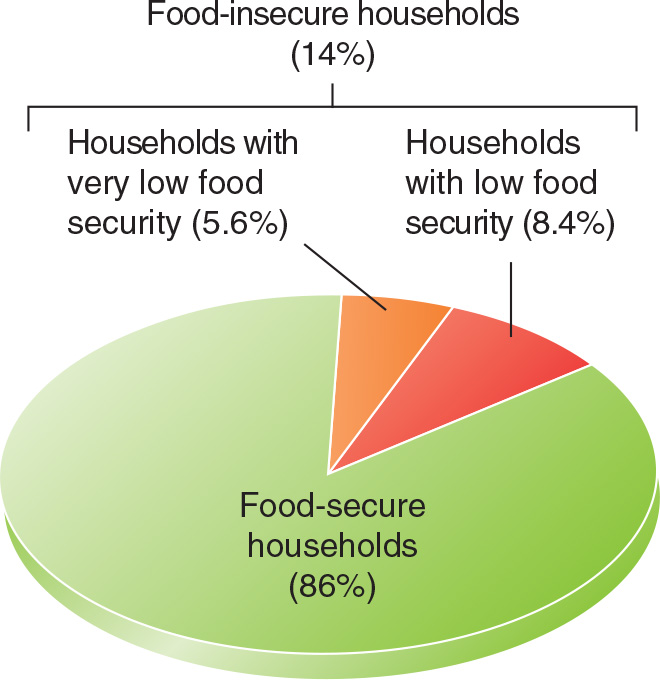
\includegraphics[width=\textwidth]{13_food_insecurity}
	\caption{Food Insecurity}
	\label{fig:food-insecurity}
\end{figure}

\section{Food Access}\label{sec:food-access}
\begin{itemize}
	\item \emph{Famine} is a severe food shortage affecting a large percentage of the population in a limited geographical area
	\begin{itemize}
		\item 20–43 million people died in the great famine in China from 1958 to 1961
	\end{itemize}
	\item \emph{Overpopulation} can occur when resources are insufficient to support the number of people living there
	\begin{itemize}
		\item Uneven distribution of food
	\end{itemize}
\end{itemize}

\section{Chronic Hunger}\label{sec:chronic-hunger}
\begin{itemize}
	\item Local conditions can contribute to chronic hunger
	\begin{itemize}
		\item \item{Cash crops}{crops grown to be sold rather than eaten, such as cotton or tobacco}
		\item Lack of infrastructure
		\item Impact of disease
	\end{itemize}
\end{itemize}

\section{Climate Change Threatens Food Security}\label{sec:climate-change-threatens-food-security}
\begin{itemize}
	\item \emph{Global warming} is the general term used for the increase of about 1.5\textdegree{}F in temperature that has occurred on the Earth’s surface over the past century.
	\begin{itemize}
		\item Many scientists believe this is due to the carbon dioxide produced by human activities
		\item A 2015 study attributed 75\% of heat extremes and 18\% of precipitation extremes to global warming
	\end{itemize}
\end{itemize}

\section{Sustainability}\label{sec:sustainability}
\begin{itemize}
	\item \emph{Sustainability} is the ability to satisfy basic economic, social, and security needs now and in the future without undermining the natural resource base and environmental quality on which life depends
	\begin{itemize}
		\item Sustainable practices can help
		\begin{itemize}
			\item Reduce pollution of soil and water
			\item Maintain or improve food diversity
			\item Reduce the number of \emph{food deserts}--geographic areas where people lack access to affordable, nutritious food
		\end{itemize}
	\end{itemize}
\end{itemize}

\begin{figure}[H]
	\centering
	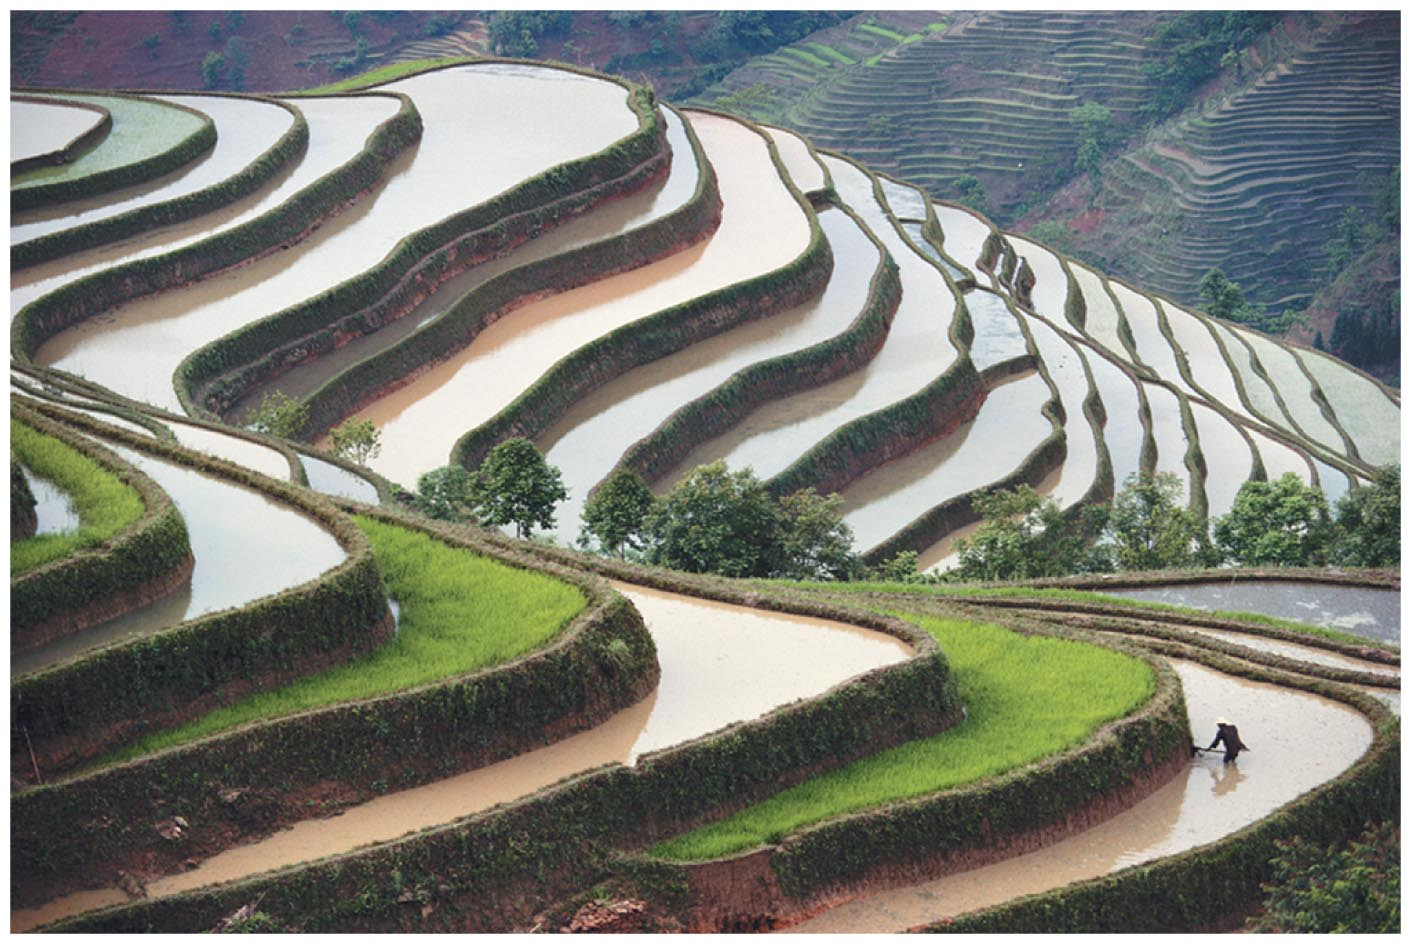
\includegraphics[width=\textwidth]{13_food_ethics_sustainability}
	\caption{Food Ethics: Sustainability}
	\label{fig:food_ethics_sustainability}
\end{figure}

\begin{itemize}
	\item Food movement initiatives that aim to promote sustainability and food diversity include
	\begin{itemize}
		\item Family farms
		\item Community supported agriculture (CSA)
		\item Farmers’ markets
		\item Urban agriculture
		\item School gardens
		\item Entrepreneurship investing in food startups
		\item Corporate involvement
	\end{itemize}
\end{itemize}

\section{Industrial Agriculture}\label{sec:industrial-agriculture}
\begin{itemize}
	\item \emph{Green Revolution}
	\begin{itemize}
		\item Massive program that has improved the technology and practices in agriculture
	\end{itemize}
	\item \emph{High yield varieties (HYVs)}
	\begin{itemize}
		\item New forms of food products (like grains) that were produced by cross-breeding plants and selecting the most desirable traits
	\end{itemize}
\end{itemize}

\section{Food Diversity}\label{sec:food-diversity}
\emph{Food diversity} is the variety of difference species of food crops available
\begin{itemize}
	\item In the 1960s the federal Agricultural Adjustment Act provided financial incentives for farmers to grow singles crops that were cultivated on a massive scale called \emph{monocultures}
\end{itemize}

\section{Food Industry Influences America’s Diet}\label{sec:food-industry-influences-americas-diet}
\begin{itemize}
	\item In 2015 lobbyists were recorded spending the following amounts to promote certain aspects of food production
	\begin{itemize}
		\item Livestock: \$2.9 million
		\item Dairy: \$7 million
		\item Sugar: \$10.3 million
		\item Food manufacturers: \$18.3 million
		\item Beer, wine, and liquor: \$25 million
	\end{itemize}
\end{itemize}

\section{International Initiatives}\label{sec:international-initiatives}
\begin{itemize}
	\item There are many international initiatives that strive to increase access to nourishing foods
	\begin{itemize}
		\item WHO and UNICEF promote breastfeeding
		\item United Nations World Food Programme
		\item USAID and Peace Corps agricultural education programs
	\end{itemize}
\end{itemize}

\section{National and Local Programs}\label{sec:national-and-local-programs}
\begin{itemize}
	\item In the United States many programs help to increase access to nourishing foods
	\begin{itemize}
		\item SNAP
		\item WIC
		\item National School Lunch and Breakfast Program
		\item USDA Commodity Food Program
		\item CDC Healthful Corner Store
	\end{itemize}
\end{itemize}

\section{Food Ethics: Food Equity}\label{sec:food-ethics:-food-equity}
\begin{itemize}
	\item \definition{Fair trade}{trading partnership promoting equity in international trading relationships and contributing to sustainable development by securing the rights of marginalized producers and workers}
	\begin{itemize}
		\item Born in response to the exploitation of farm laborers around the world
		\item Depends on support from consumers purchasing Fair Trade products
	\end{itemize}
	\item \definition{Food equity}{sharing the world’s food and other resources fairly}
	\begin{itemize}
		\item One in seven people in the world is chronically undernourished, almost all of them in developing nations
		\item The major cause of undernutrition is unequal distribution of food because of poverty
	\end{itemize}
\end{itemize}

\begin{figure}[H]
	\centering
	
\includegraphics[width=\textwidth]{13_fair_trade_certified}
	\caption{Food Ethics: Food Equity}
	\label{fig:13_food_ethics_food_equity}
\end{figure}

\section{Choose Foods That Are Healthful for You}\label{sec:choose-foods-that-are-healthful-for-you}
\begin{itemize}
	\item Buy organic or reduce synthetic pesticide use
	\item Purchase local produce and support local economy
	\item Choose whole foods or less processed foods
	\item Avoid empty Calorie foods and beverages
	\item When eating out ask for nutrition information
\end{itemize}

\section{In Depth: Malnutrition}\label{sec:in-depth:-malnutrition}
\begin{itemize}
	\item Approximately 51 million children do not weigh enough for their height
	\item Severe acute malnutrition (SAM)\label{dfn:sam}
	\begin{itemize}
		\item Condition in which energy intake is so inadequate that the child experiences a lower body weight than normal
	\end{itemize}
	\item Approximately 161 million children experience \emph{stunted growth} which causes them to be shorter than expected for their age.
	\item SAM dramatically increases a population’s rate of :
	\begin{description}
		\item[Maternal mortality:] deaths of a woman during pregnancy, childbirth, or in the immediate postpartal period
		\item[Infant mortality:] deaths of infants between birth and 1 year of age
	\end{description}
	\item Micronutrient deficiencies can lead to preventable diseases
	\begin{itemize}
		\item Iron deficiency anemia (most common deficiency worldwide)
		\item Prenatal iodine for fetal brain development
		\item Vitamin A deficiency is the leading cause of blindness in children
	\end{itemize}
\end{itemize}

\begin{figure}[H]
	\centering
	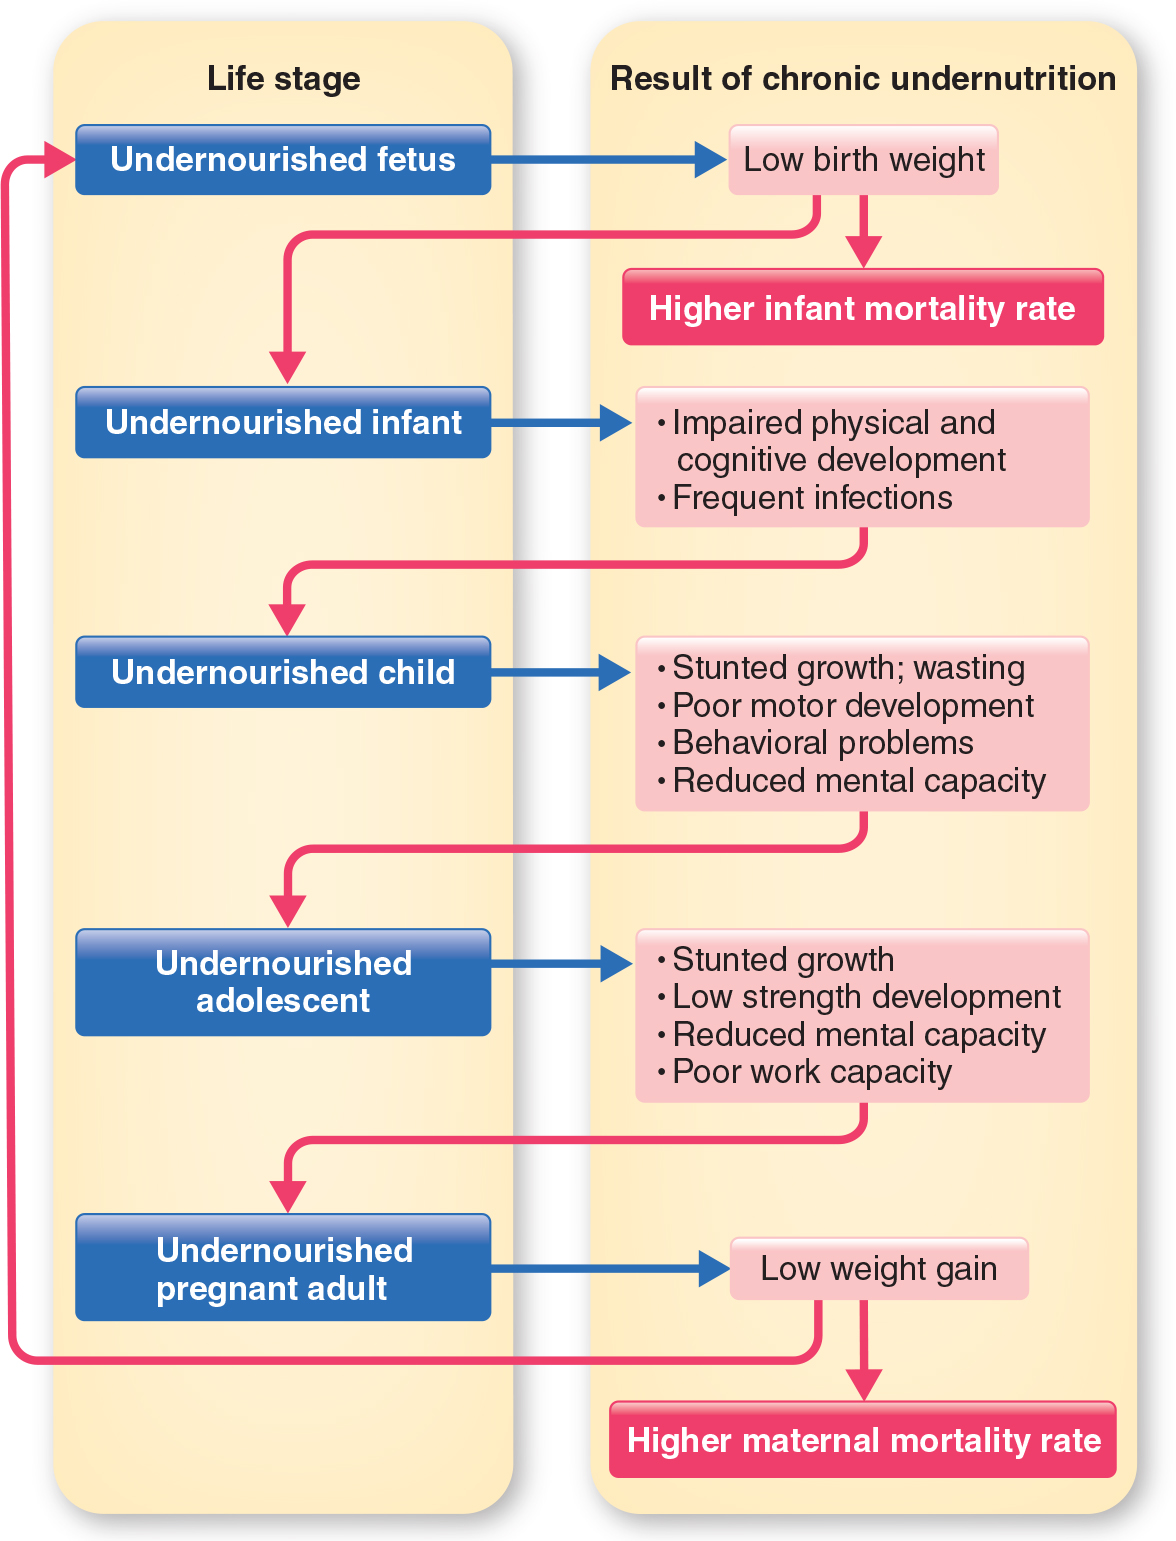
\includegraphics[width=\textwidth]{13_malnutrition}
	\caption{Malnutrition}
	\label{fig:malnutrition}
\end{figure}

\begin{itemize}
	\item \emph{Nutrition paradox} is characterized by the coexistence of stunting and overweight/obesity within the same region, the same household, and even the same person
	\begin{itemize}
		\item The WHO identifies two key factors:
		\begin{itemize}
			\item A trend toward decreased physical activity
			\item A global shift toward increased consumption of energy dense foods
		\end{itemize}
	\end{itemize}
	\item Poverty-obesity paradox occurs when obesity is more prevalent in low-income populations
	\begin{itemize}
		\item Some researchers have also observed a so-called \emph{hunger-obesity paradox} in which low income people are obese while also deficient in one or more nutrients
	\end{itemize}
	\item \emph{Food deserts} also contribute to malnutrition and poor food access
	\begin{itemize}
		\item Characterized as geographic areas where people lack access to fresh, healthful, and affordable food
	\end{itemize}
\end{itemize}

%</Chapter13>

\end{document}
